\chapter*{Introdução}	% Completar
\addcontentsline{toc}{chapter}{Introdução}
\label{introducao}

Como parte da disciplina Projetos de Aeronaves I, do curso de Engenharia Aeroespacial, da Universidade Federal de Minas Gerais, pretende-se realizar o projeto de uma aeronave que compreende os seguintes aspectos:

\begin{itemize}
  \item Aerodinâmica;
  \item Desempenho;
  \item Estabilidade e Controle;
  \item Propulsão;
  \item Estimativa de Peso;
  \item Análise Estrutural;
  \item Regulamentos Aeronáuticos.
\end{itemize}

A divisão proposta das fases de projeto é definida de acordo com \cite{gudmundsson}, sendo que o escopo deste relatório abrange a primeira etapa e parcialmente a segunda etapa listadas a seguir:

\begin{enumerate}
  \item Definição de Requisitos;
  \item Estudos Conceituais;
  \item Estudos Preliminares;
  \item Projeto Detalhado;
  \item Fabricação da aeronave e ensaios.
\end{enumerate}

O produto final da etapa \emph{Definição de Requisitos} compreende uma lista de expectativas técnicas que a aeronave deve atender.
Nesta lista de requisitos, tem-se itens derivados de diretrizes gerais dadas para o projeto da aeronave pelo professor responsável, além de requisitos de alto nível definidos a partir de tabela comparativa e estudo de mercado das principais aeronaves em serviço atualmente na aviação regional.

As diretrizes gerais para a aeronave são:

\begin{itemize}
  \item Aeronave de transporte;
  \item Número de passageiros em torno de 50, sendo que a aeronave poderá ser capaz de transportar no mínimo 30 e no máximo 70 passageiros;
  \item Velocidade máxima deve ser no mínimo \si{650}{km/h};
  \item Teto máximo de operação deve ser no mínimo de \si{7000}{m}.
\end{itemize}

Além disso, tem-se o perfil de missão típica que a aeronave deve ser capaz de realizar de forma eficiente (\autoref{fig:MISSAOGENERICA}).
Os parâmetros necessários para definir o cruzeiro típico serão discutidos ao longo do relatório.
Já o tempo máximo da missão é definido como 3 horas. Ou seja, a aeronave a ser projetada deverá ser classificada como \emph{short-haul}.

\begin{figure}
\centering
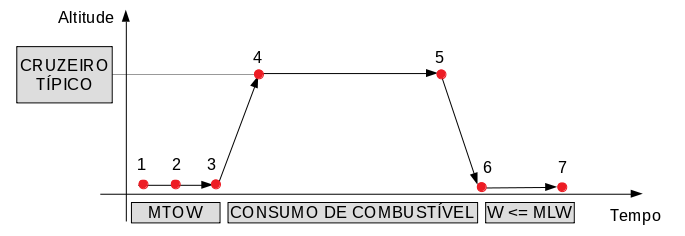
\includegraphics[width=120mm]{images/parte1/MISSAO_GENERICA}
\caption[Perfil de missão típica]{Perfil de missão típica. MTOW é o peso máximo de decolagem e MLW é o peso máximo para pouso.}
\label{fig:MISSAOGENERICA}
\end{figure}

O propósito deste trabalho é desenvolver o projeto de uma aeronave que seja a melhor em sua categoria.
De início, o objetivo será apresentar um projeto competitivo em todos os aspectos.
Sabe-se que alguns requisitos e objetivos podem ser conflitantes.
Portanto, como parte dos estudos conceituais, alguns aspectos serão priorizados de forma a ainda garantir uma aeronave competitiva em sua categoria.

%Outline
A partir do objetivo do projeto e do escopo deste relatório, a metodologia foi estruturada com a finalidade de definir os requisitos de projeto e de apresentar um esboço inicial da aeronave.

Para a primeira atividade apresentada no \autoref{tabelacomparativa}, decidiu-se analisar as aeronaves que atendem as diretrizes gerais listadas anteriormente e que estão em serviço, mesmo que não mais em produção, por meio de uma tabela comparativa \cite{barros}.
Neste momento, tem-se como objetivo mapear quais são as características de desempenho médias encontradas nessa categoria, bem como as soluções de projeto que compreendem, por exemplo, a definição do grupo moto-propulsor.

O próximo passo é a análise de mercado, que tem como propósito identificar quais são as características de desempenho apresentadas pelas aeronaves competitivas e quais são as exigências do mercado na aviação comercial.
O resultado desta última atividade é apresentado no \autoref{mercado}.

Já na \autoref{requisitos}, discute-se quais são os requisitos adotados de forma a garantir o projeto da melhor aeronave da categoria. Na \autoref{esbocoinicial}, tem-se um esboço inicial para a aeronave a ser projetada com base nos requisitos estabelecidos levando em consideração geometria externa e ergonomia. Por fim, no \autoref{conclusao} conclui-se em relação aos resultados obtidos, os requisitos e o esboço inicial da aeronave.
